\documentclass[a4paper,11pt]{article}

\usepackage[utf8]{inputenc}
\usepackage{graphicx}
\usepackage{epsfig}
\usepackage[italian]{babel}
\usepackage{listings}
\usepackage{hyperref}
\usepackage{authblk}
\usepackage{fancyhdr}
\usepackage{floatflt}
\usepackage{caption}
\usepackage{wrapfig}
\usepackage{rotating}
\usepackage{longtable}
\usepackage{chngcntr}
\usepackage{relsize}
\usepackage{amsmath}
\usepackage[a4paper,top=3cm,bottom=3cm,left=1.8cm,right=1.8cm]{geometry}

\usepackage{appendix}    
\usepackage{pdfpages}


\pagestyle{fancy}
\setlength\headheight{13.6pt}
\fancyhf{}
\rhead{Logbook - Nicolò Foppiani, Tommaso Pajero}
\lhead{\rightmark}
\rfoot{\thepage}
\lfoot{Summer stage at CERN 2015}

%opening
\title{Summer CERN stage Logbook}
\author{Nicolò Foppiani, Tommaso Pajero}
\affil{\href{http://www.df.unipi.it}{Università degli studi di Pisa}}
\affil{\href{http://www.sns.it}{Scuola Normale Superiore}}
\date{\today}

%Numerazione reset ogni section
\counterwithin{figure}{section}
\counterwithin{equation}{section}
\counterwithin{table}{section}

\begin{document}

\maketitle

\newpage

\tableofcontents

\newpage

\section{Week 01}
\subsection{20/07/2015}

\textbf{Access to Cern}

The first day we did a lot of bureaucracy. It's not necessary to register the car, our badge permits us to pass.
During the afternoon we have attended to a conference during which our tutors have presented the projects.


\subsection{21/07/2015}

\textbf{First use of Castor and Marlin}

\textbf{Kinematics}

The first process we analyze is the $e^+ e^- \to t \bar{t} $ with energy $\sqrt{s}=365$ Gev, where one top decays as $t \to bW \quad W \to l\nu$, and the other top in three jets. This process with two leptons are more rare, while, on the other and, the process with 6 jets are really difficult to study.

By analyzing the kinematics of the process we have found that the lepton has to cut in energy:
the configuration with the minimum energy is when the W has the maximum energy (emitted in the top direction) and the lepton is emitted back respect to the W fly direction;
the configuration with the maximum energy is when the W has the maximum energy (emitted in the top direction) and the lepton is emitted front respect to the W fly direction.

With the top energy of 182.5 Gev we obtain a minimum energy of 13.45 Gev and a maximum energy of 120.16 Gev. 

Anyway there will be a lot of background to this process (also with high energy) due to the lepton produced by gamma pair production or pions decays.

\subsection{22/07/2015}

\textbf{PyROOT and Git}

Installing PyRoot and Git, and created a Git repository. You can find some useful files in the utilities folder.

\subsection{23/07/2015}

\textbf{Tree Root}

Thanks to Maurizio we understood a lot about Root trees. They are like tables: the rows represent the events, the columns are the branches and contain the information of the events. 

Trees are contained in a ROOT file, to see the content we could use ROOT as follow:
root -l myfile.root
\_file0->ls()

To see a tree we can use the command:
mytree->Scan()
and it permits to see it as a table.

To loop on a tree using C++ we have to create the class associated to the tree by using:
mytree->MakeClass("myclass")
This command creates the file myclass.h that contains the definition of the class with the basic methods. The class contains some variables and the pointers to the branches.
The file myclass.C is a ROOT macro, with the function loop, which loops on the events of the tree: you can add your code in this function and make the loop by executing this macro.

In python it's more simple, because one can open the ROOT file and load the tree by using 

myfile = TFile("myfile.root","READ")
mytree = file.Get("mytree")

and then, to loop on the events of the tree

for event in mytree:
	my code

\textbf{Grow space in Lxplus}

Thanks to Maurizio we have also increased our free space on Lxplus and adopted the CMSSW\_7\_4\_7 environment to use Root macro on Lxplus. See the file configurazioneLXPlus.txt in utilities to find some useful commands.

\subsection{24/07/2015}

\textbf{Using Pyroot scripts}

We have started writing python scripts. At the end of the script, all the canvas opened are automatically closed, so, to save the histograms and plots the best way is to save them into a Root file.
Here is an example.

file\_to\_save1 = TFile("./file\_to\_save1.root","CREATE")
Part\_ID.Write()

where PartID is a TCanvas variable.

We can also launch Python script using

python -i myscript.py 

which don't close the prompt at the end of the macro.

\textbf{Glob}

A useful command in Python is Glob, which gives an array of the files in one folder; we could then loop on this array.

It's also useful to keep the bash library on Python by importin os library.

\textbf{SLCIO Marlin ntuples}

We understood something more about the ntuple produced by Marlin. 

mcpdg contains the ID of the simulated particles.

mcgst contains the status of the particles. There are 4 status possible: 0, 1, 2, 102
we have understood that the particles in final state (which are revealed by the detectors) have status 1, while particles which decay have status 2. bottom quarks have status 0 and we will check later which particles have status 102.

mcmox,y,z are the three components of the momentum of the particle
mcvtx,y,z are the vertex coordinates where the particle is produced

We understood that there are lot of muons and electrons (also reconstructed) which are not produced in the W decay. They are produced, for instance, by the electrons which radiate. This effect creates a background to the leptons we want to study.
In addition the leptons we want to study can radiate and it's difficult to reconstruct these leptons. Maybe, during the study of the montecarlo events, we could analyze the vertex in which the leptons are produced.

We need to ask Patrick and Patrizia if they prefer to import all ROOT library (like import ROOT as RT) or only the functions we need in that macro.

We need also to ask them if they prefer to write a logbook with us or by themselves.

We produced a few plots of the electrons and muons energy in both reconstructed and simulated events. We need to talk about them with Patrick and Patrizia. We need also to understand how the events were smiulated (for instance if each event is only one collision or a collision between two bunches).

\section{Week 02}

\subsection{27/07/2015}

\textbf{Stage and copy file from CERN servers}

Patrick have copied all the .slcio files in his directory and processed them with Marlin using two bash scripts. We have copied the ntuples from eos (see the glossary) to our folder, and now we can loop among them. 

He used two files: jobCopy.sh and jobMarlin.sh to process the files.

jobCopy first stage the files from the tape (Castor) to the disk, and then copies the files into EOS folder.
jobMarlin loops above all the files writing the correct steering.xml file and create all the ntuple.

\textbf{More about the slcio ntuples}

We have found out something else about our ntuples: 

We discovered that all the top quark have status 3, and the bottoms have sometimes status 2 and sometimes status 3.

By using the parent information (mcpa0 e mcpa1, for daughters mcda0,1,2,3,4) we managed to select only the leptons which come from the W decay. Then, with a pyroot macro we filled the 2-D histograms of the number of leptons versus the energy and the angle.


\subsection{28/07/2015}

\textbf{Lepton vs energy-angle histogram}

We managed to loop above all the .root files. We use 256 bins (16 for the angle and 16 for the energy), that are quite similar to the square root of the entries (they are about 40k, the 40\% of 100k events).\\
We have also used the reduced energy defined as \[x=\frac{2E}{m_t} \sqrt{\frac{1-\beta}{1+\beta}} \]   \[ \beta =\sqrt{1-4m_t^2/s} \]
We plotted the histo of the number of lepton in function of the $cos(\theta)$ and of the reduced energy. We expected a curve distribution in both the variables, and, to do this, we have to plot only the positive leptons (or the negative); otherwise there can't be any asymmetry in the angular distribution.

The result can be seen in figure \ref{02_Electrons}, \ref{02_Muons}, \ref{02_Electrons+muons}

\begin{figure} [ht!]
  \centering
  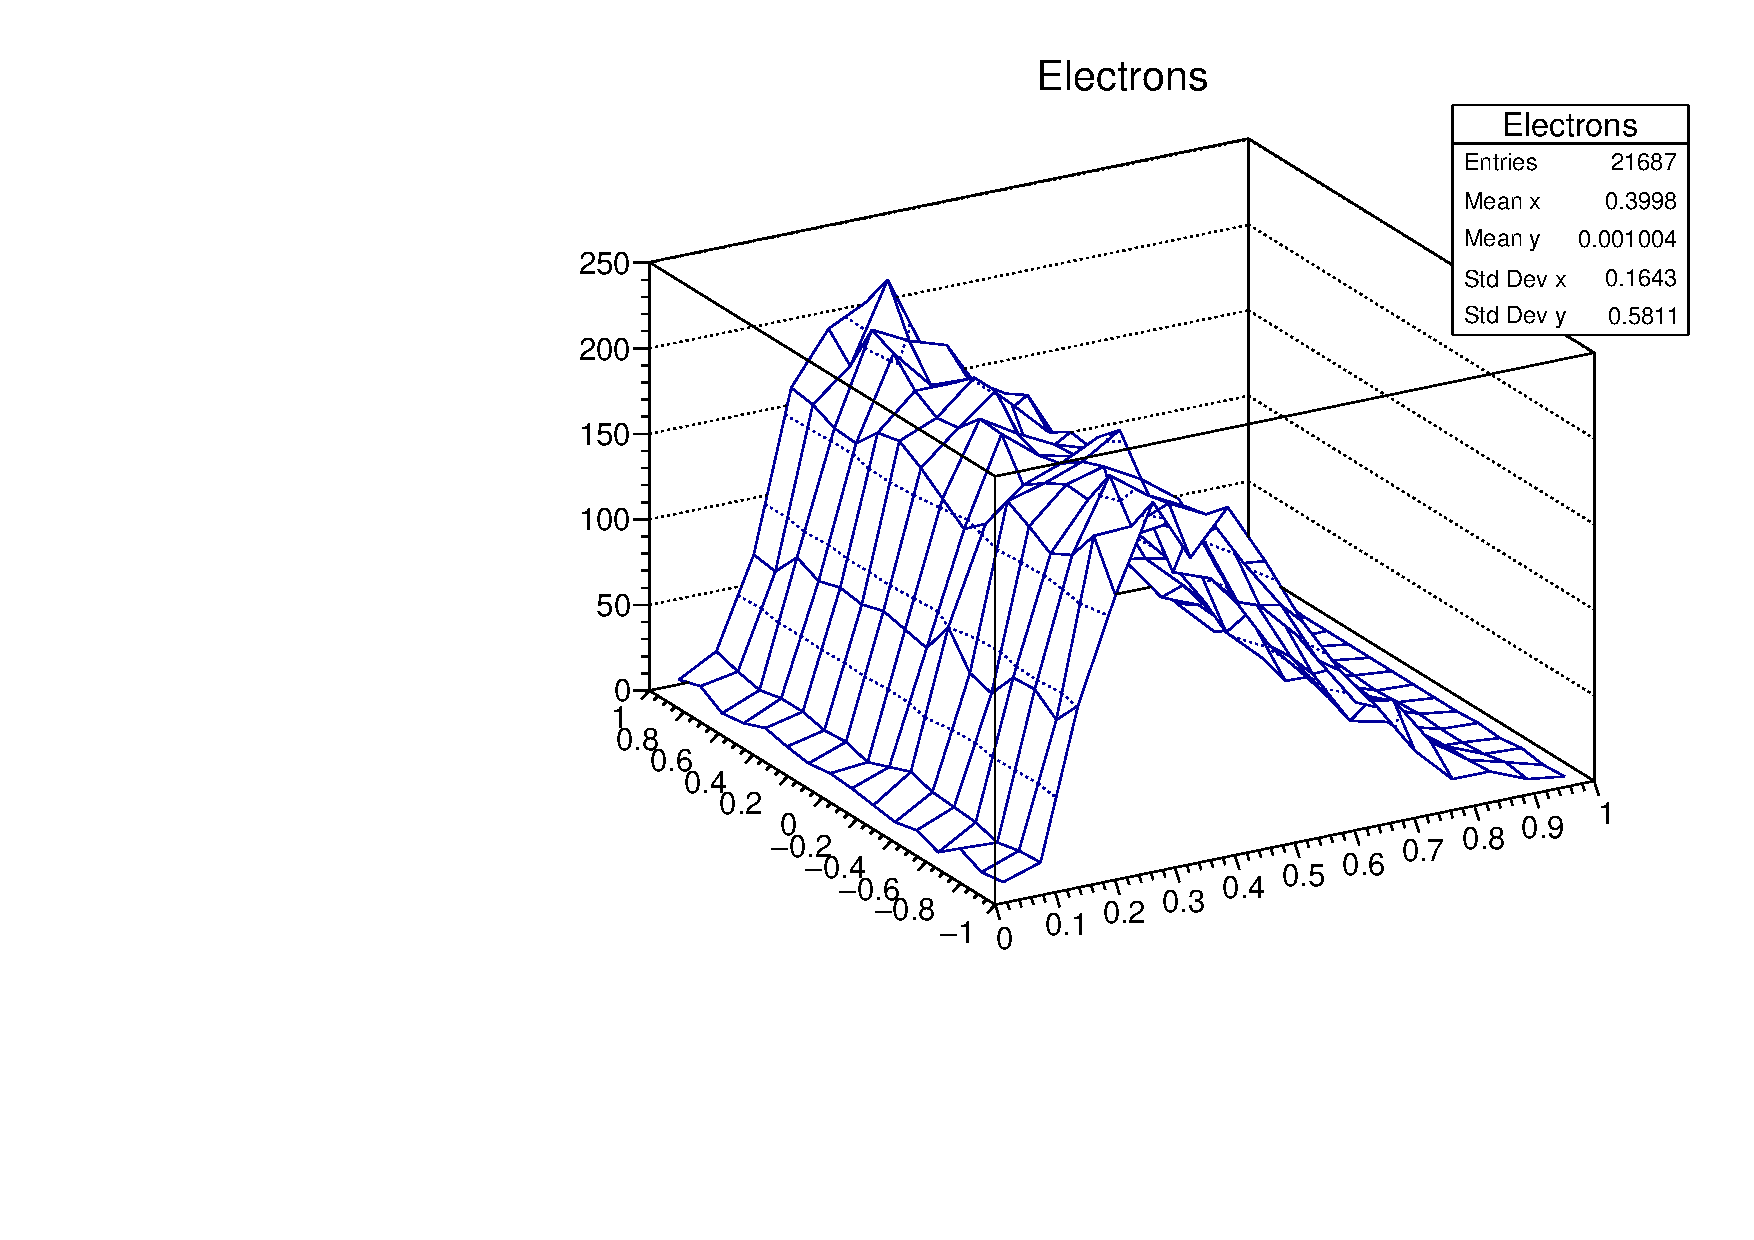
\includegraphics[width=0.7\textwidth]{02_Electrons.pdf}
 \caption{Energy-angle distribution of the electrons}
 \label{02_Electrons}
\end{figure}

\begin{figure} [ht!]
  \centering
  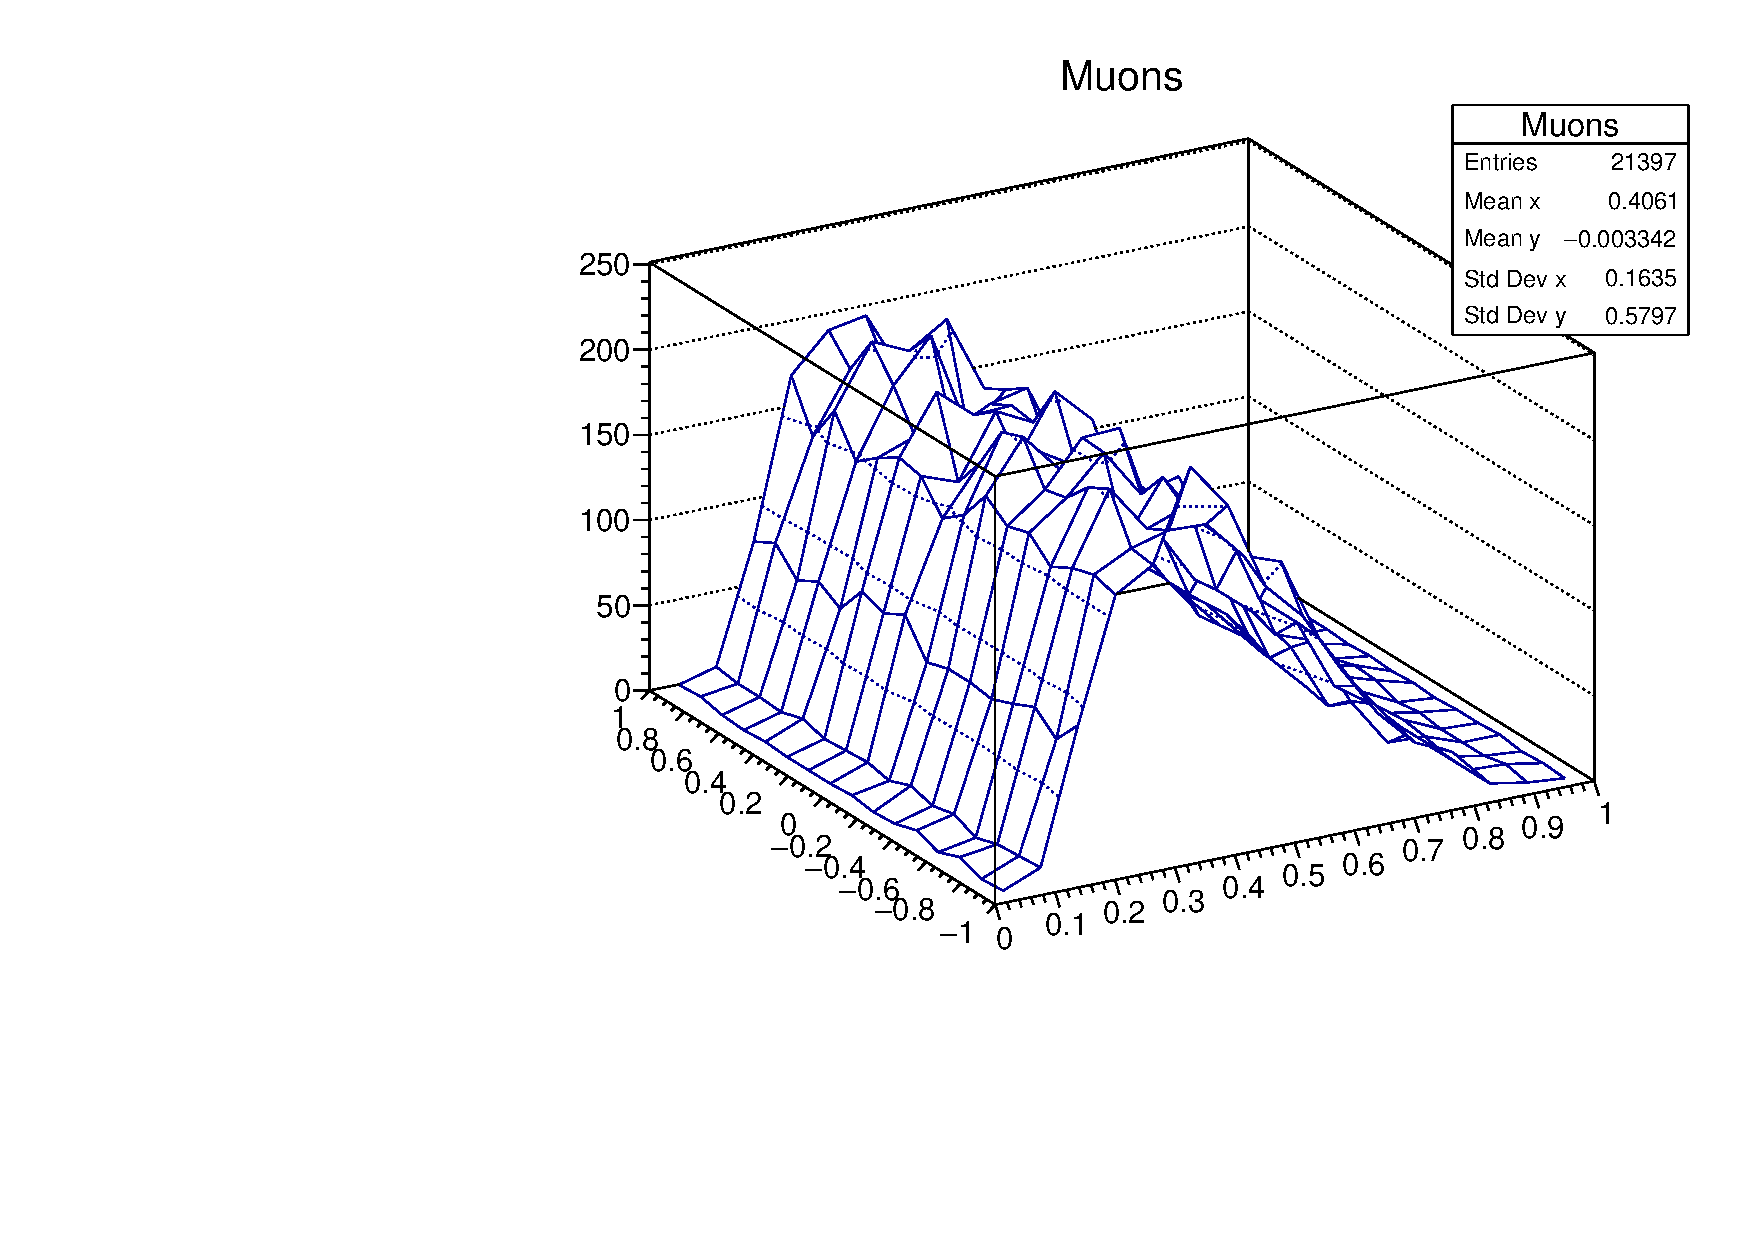
\includegraphics[width=0.7\textwidth]{02_Muons.pdf}
 \caption{Energy-angle distribution of the negative muons}
 \label{02_Muons}
\end{figure}

\begin{figure} [ht!]
  \centering
  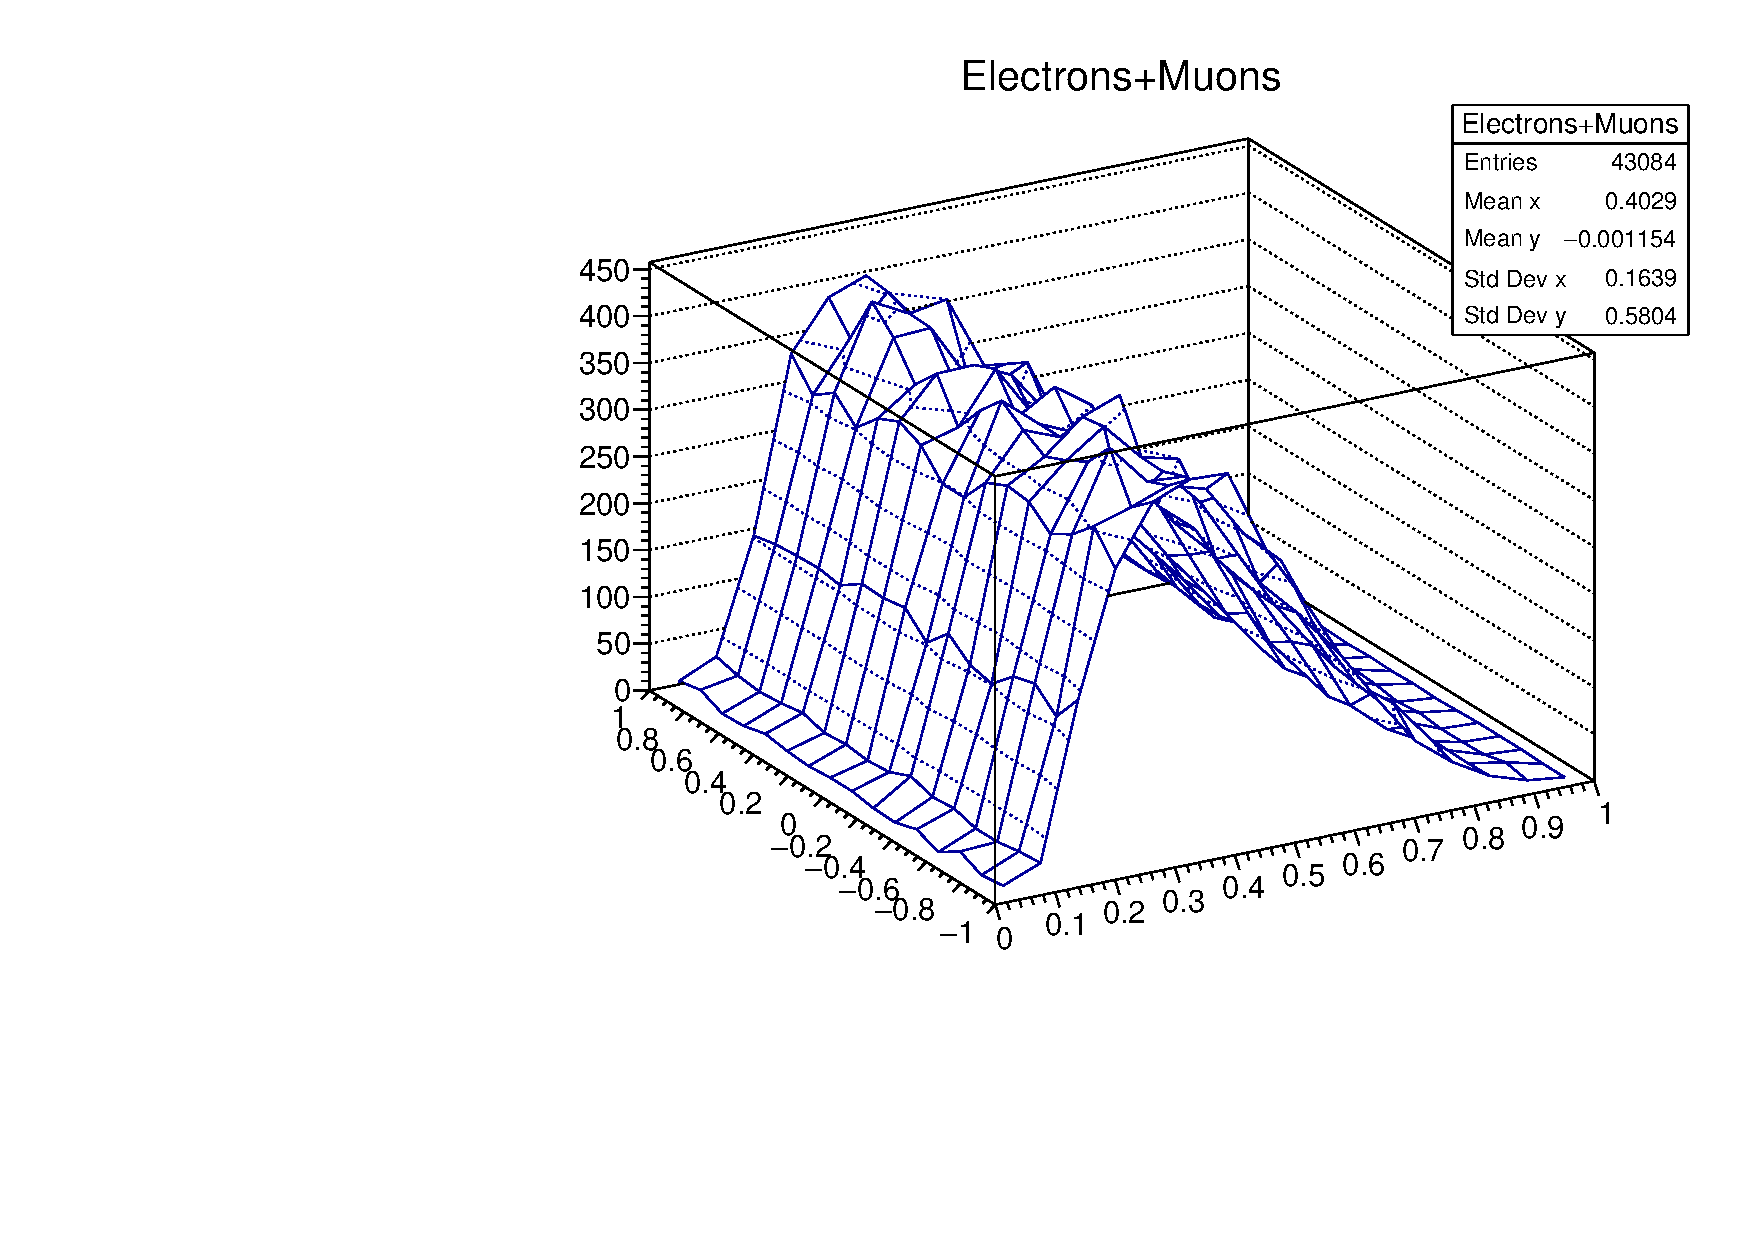
\includegraphics[width=0.7\textwidth]{02_Electrons+muons.pdf}
 \caption{Energy-angle distribution of the electrons and negative muons}
 \label{02_Electrons+muons}
\end{figure}

Unfortunately the angular distribution is flat: this implies that Pythia simulation don't consider the top polarization. So we cannot use these simulation to perform our analysis, and we need to proceed with different data.

\textbf{Writing Root Tree using PyROOT}

We have also learn how to write a Tree Root using PyROOT. We need first to define a TTree variable, then define the branches, and then fill the branches with a 0-D array (this is important), by looping on the events.
Further information in the glossary folder.

\subsection{29/07/2015}

\textbf{Copy and Marlin new simulation files}

We decided to use other simulation files made with Wizard (instead that Pythia), we could find them at this site \href{https://twiki.cern.ch/twiki/bin/view/CLIC/MonteCarloSamplesForTopPhysics?sortcol=2;table=3;up=1#sorted_table.}{clicca qui}
These simulations are made at 365 GeV and would consider the polarization of the top quarks (we hope so).

By using some scripts bash we have staged all the files, copied and Marlin them.

\subsection{30/07/2015}

\textbf{Whizard ntuples}

We have started to analyze the new ntuples obtained with Whizard simulation. The tree branches have the same name. Though we found out that all the events contains the following particles:
0,1 : the two incoming electrons
2,3 : the two incoming electrons after radiating soft photons
4,5 : the two soft photons
6,7,8,9,10,11 : the final state of the event with b an $\bar{b}$ quark, a couple quark and anti-quark, the electron (positron) we are looking for with index 10 and the correspondent neutrino.

So we have simply plotted the distribution of the electron with index 10 and we found out that the angular distribution has the asymmetry we are looking for.\\
Now we are going to run our script on lxplus looping all the data.

In addition we discover that we have not always the resonant state in the simulation, and sometimes we have a top without an antitop (or viceversa); so we don't know very well how the simulation was made. We don't care to this fact very much for the moment. 

\subsection{31/07/2015}

\textbf{Whizard ntuples}

The result of the plot with all date is visible in figure \ref{02_Energy_angle_MC}.

\begin{figure} [ht!]
  \centering
  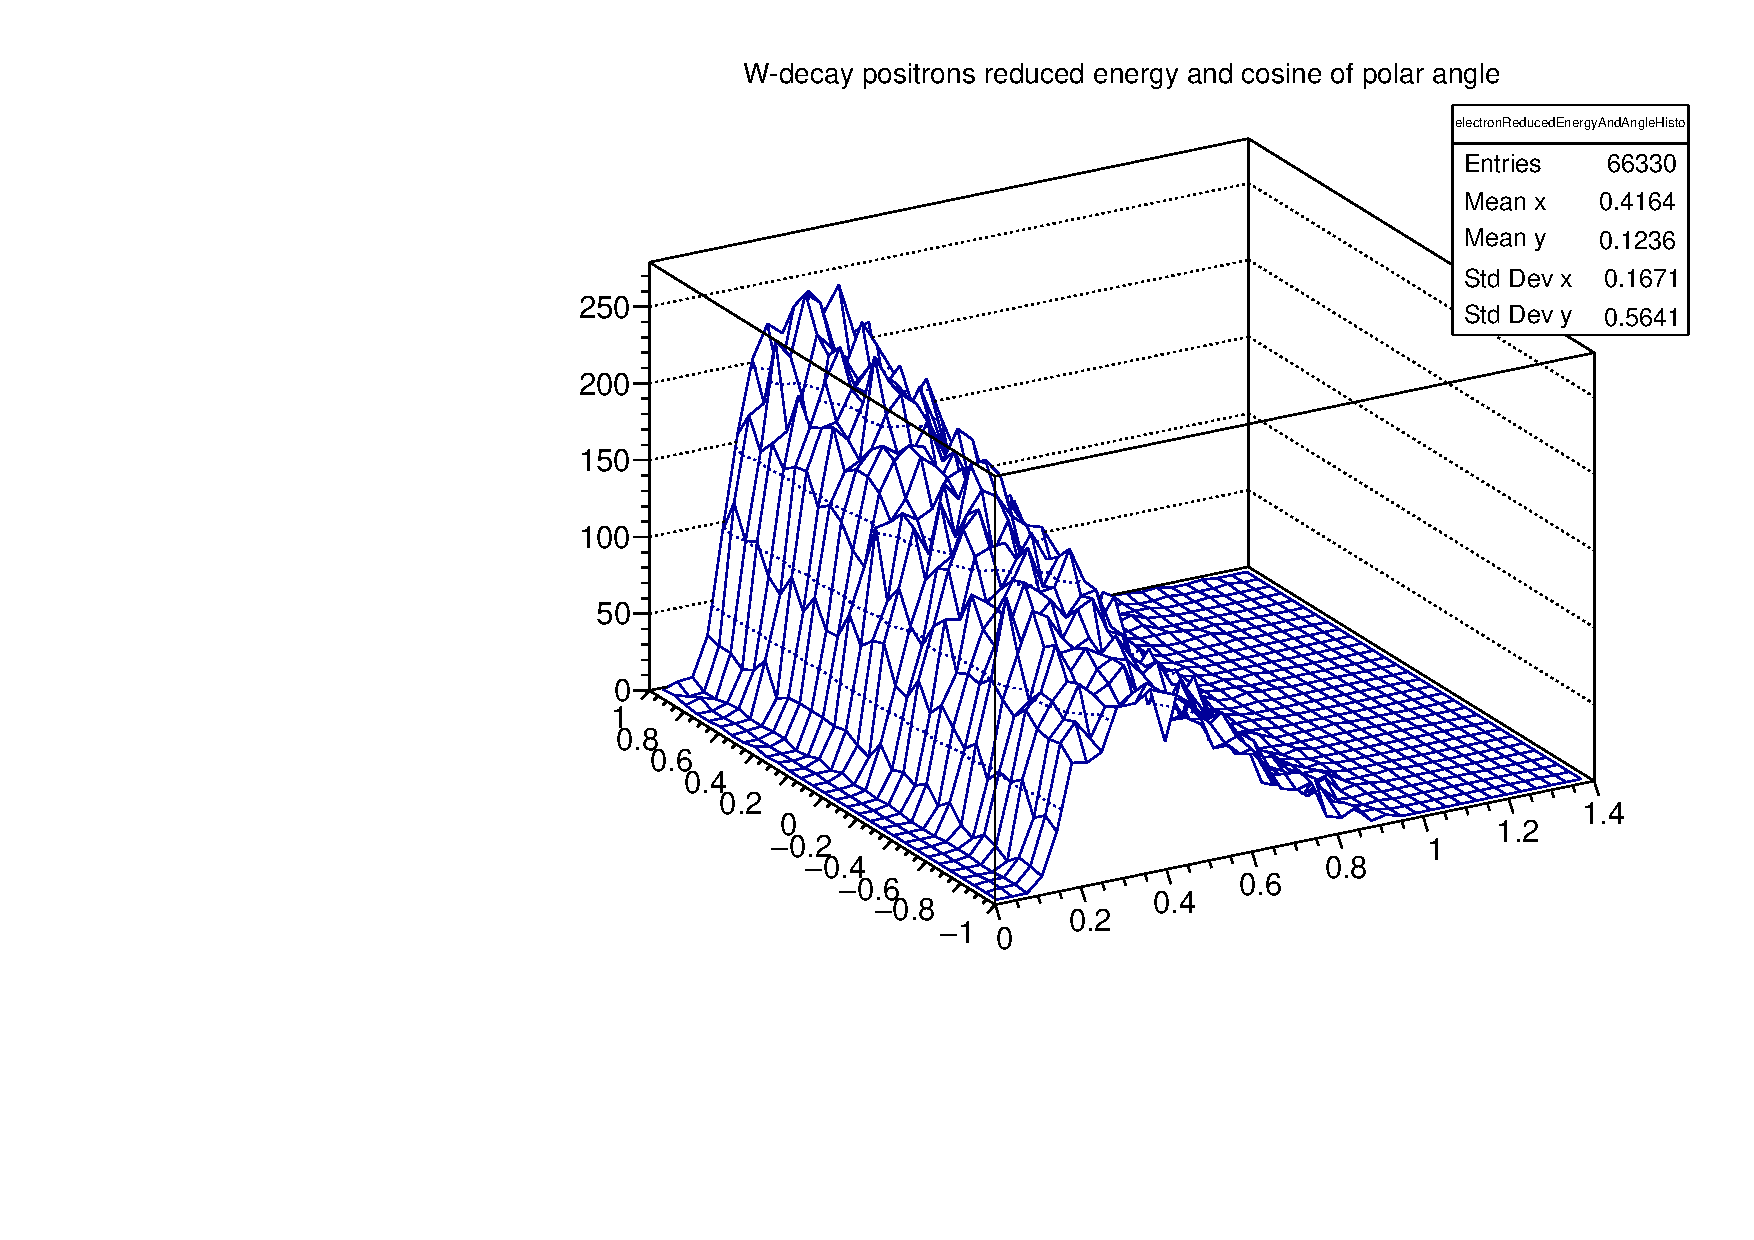
\includegraphics[width=0.7\textwidth]{02_Montecarlo_electron_distribution.pdf}
 \caption{Energy-angle distribution of the electrons simulated by Whizard}
 \label{02_Energy_angle_MC}
\end{figure}

We have then compared this distribution with the one calculated analytically (figure \ref{02_Energy_angle_AN}), and, by making the ratio of the two histograms we obtained something really flat (figure \ref{02_Energy_angle_ratio}), so the two distributions agree. There are some spike in the ratio of the two histograms near the boundary of the allowed energy. This is due to the fact that probably the top mass and the W mass were chosen approximately (we found out that the top mass were chosen to be 174 GeV), and the maximum energy of the electrons depends a lot on the top mass.

\begin{figure} [ht!]
  \centering
  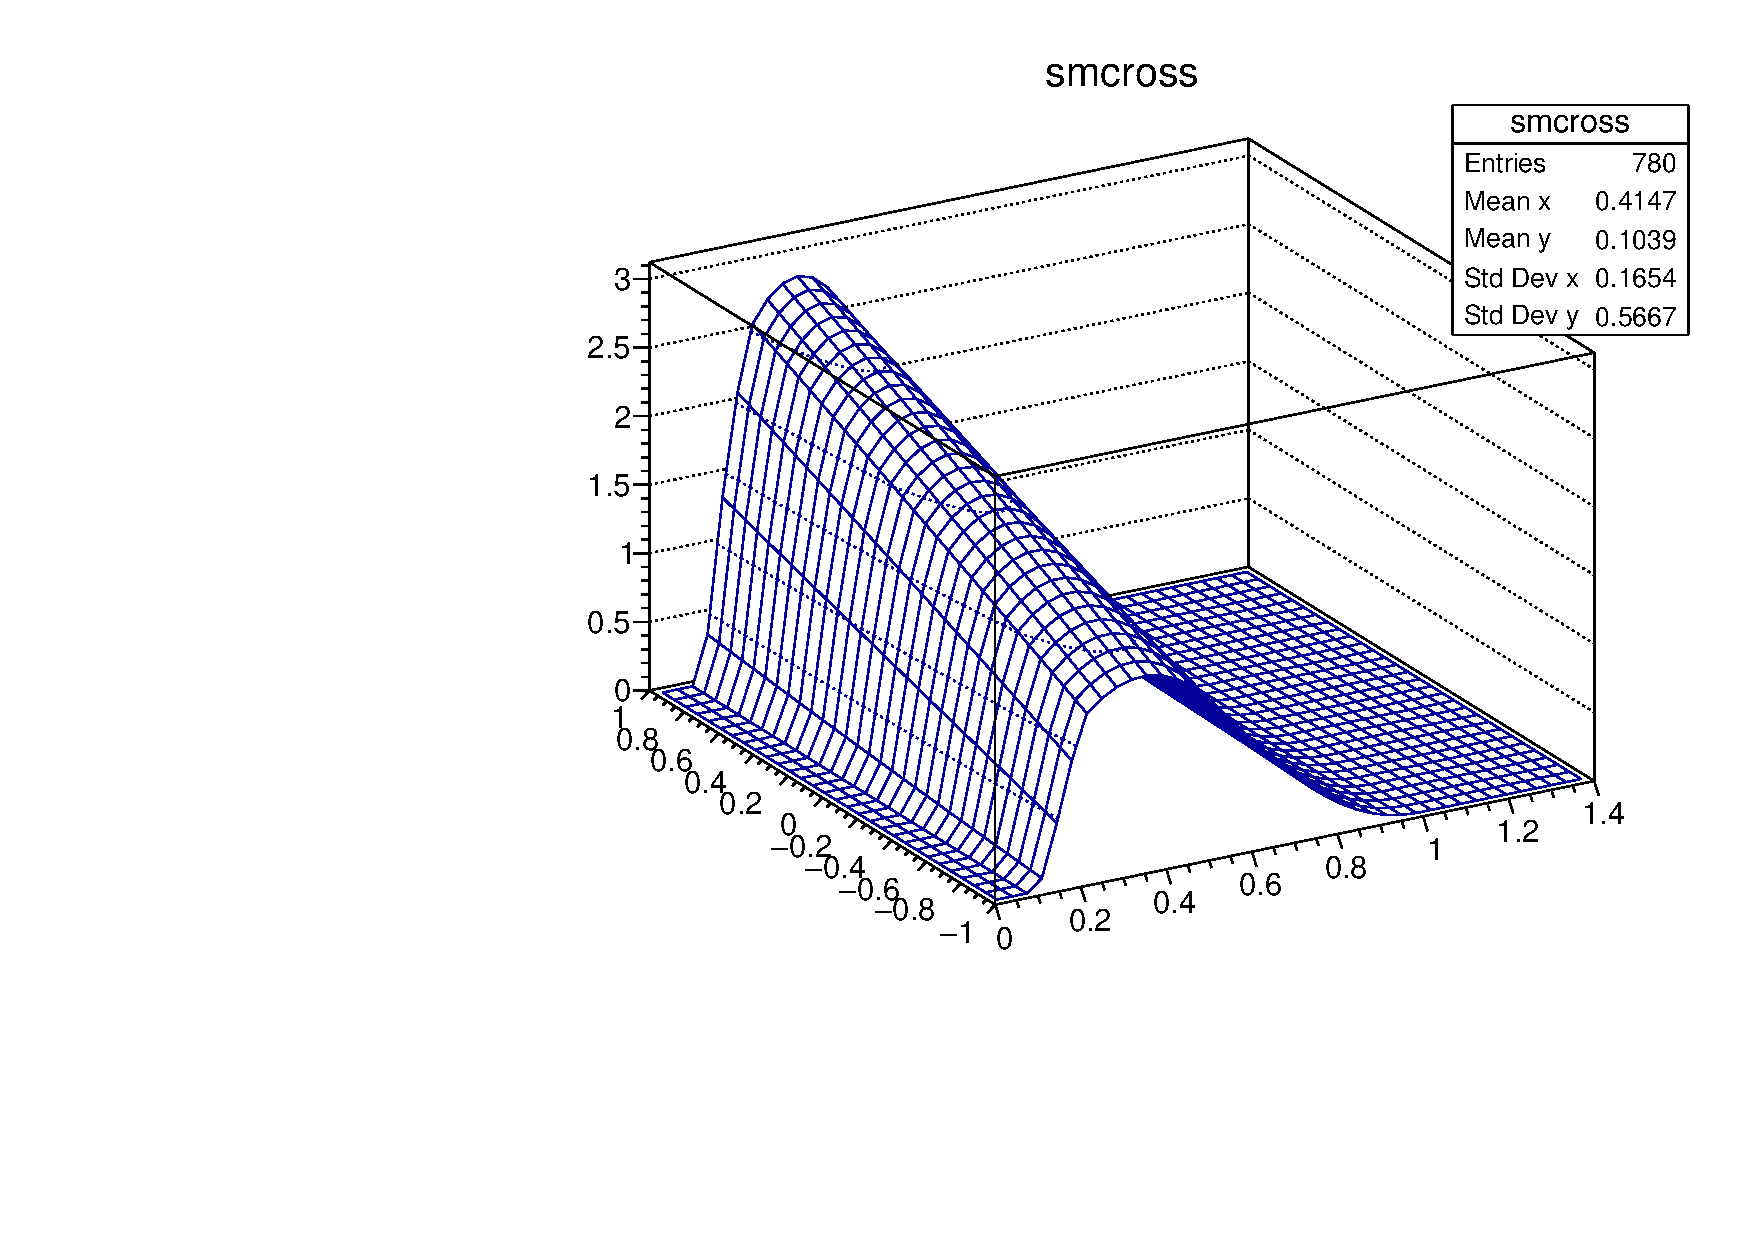
\includegraphics[width=0.7\textwidth]{02_Analytic_electron__distribution.pdf}
 \caption{Energy-angle distribution of the electrons calculated analytically}
 \label{02_Energy_angle_AN}
\end{figure}

\begin{figure} [ht!]
  \centering
  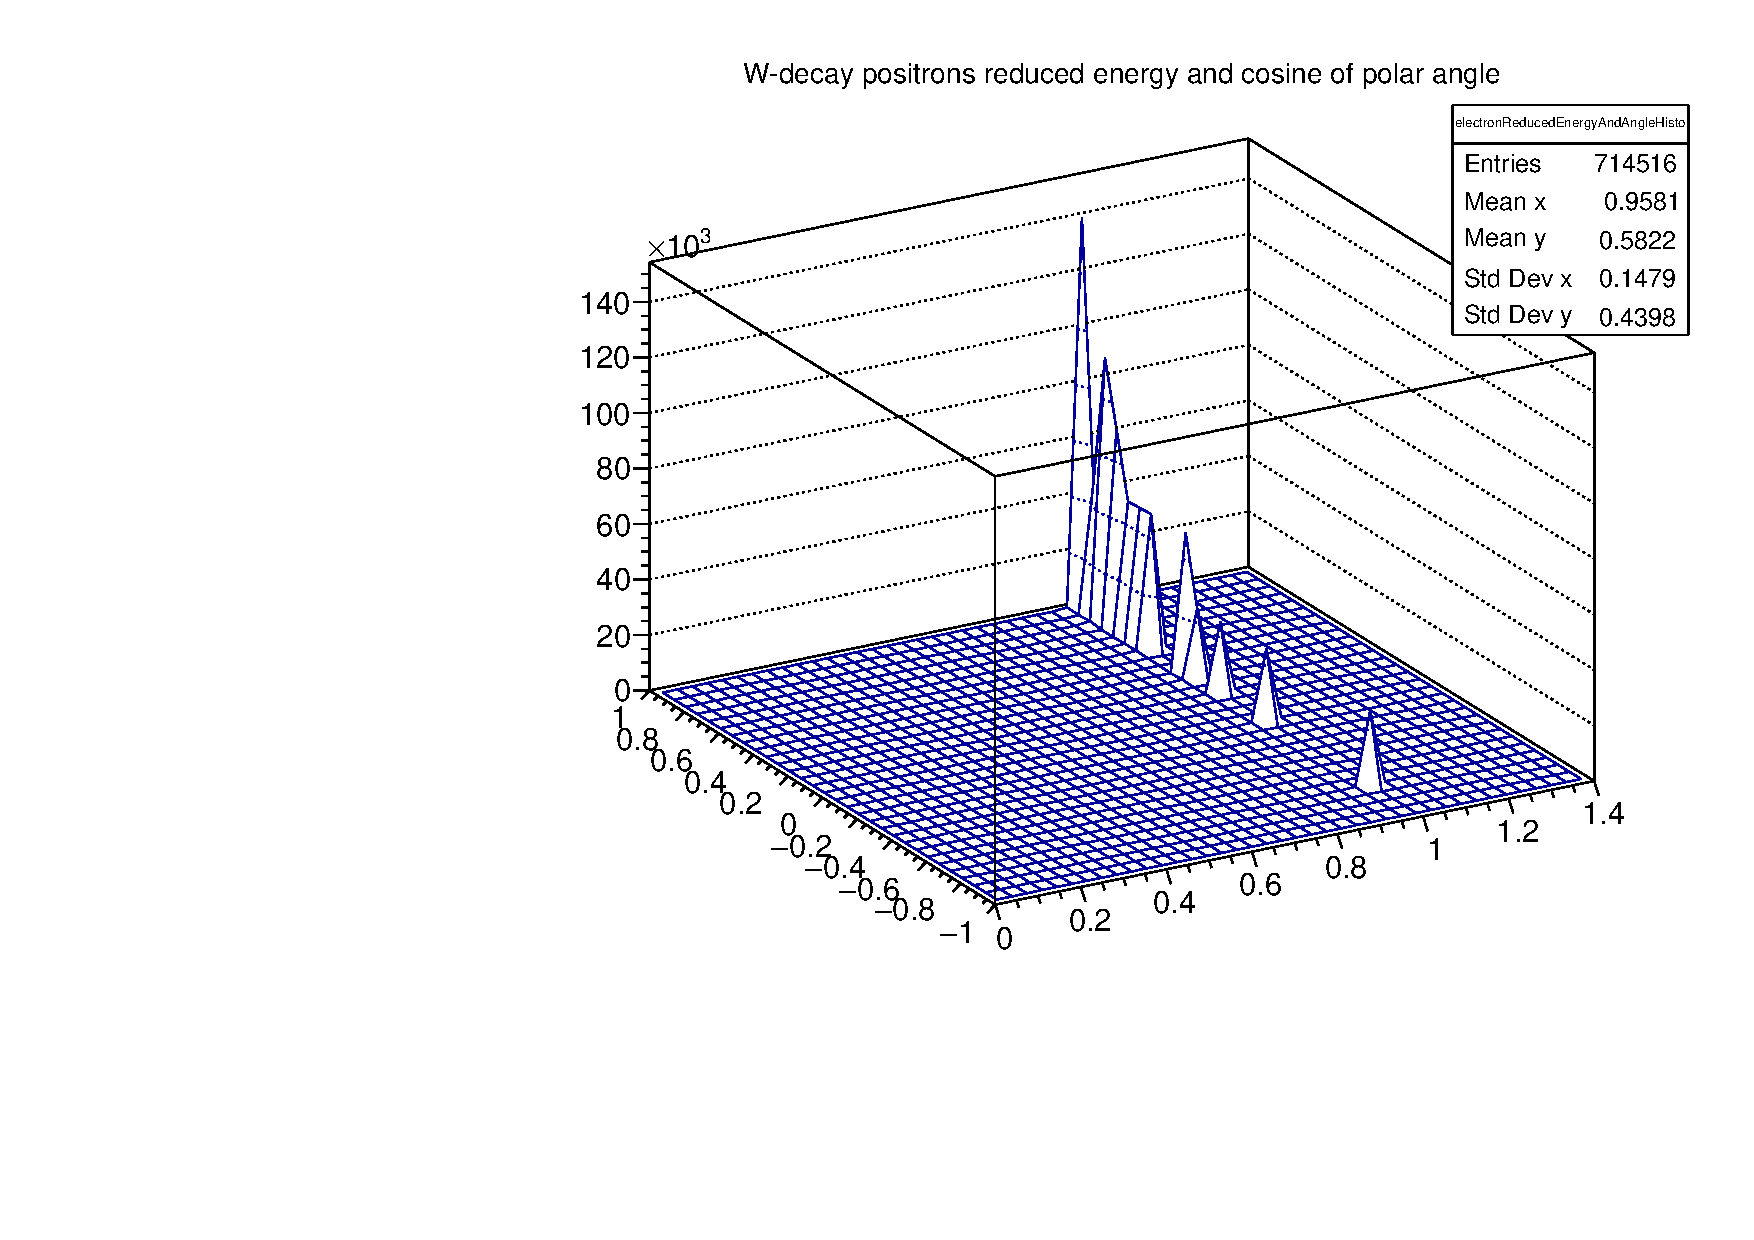
\includegraphics[width=0.7\textwidth]{02_Ratio_MC_An.pdf}
 \caption{Ratio of the distribution simulated and analytic}
 \label{02_Energy_angle_ratio}
\end{figure}

If we better analyze the ratio by zooming on the distribution in the flat region, we can see that there are many fluctuations that are due to the little quantity of data. 

\begin{figure} [ht!]
  \centering
  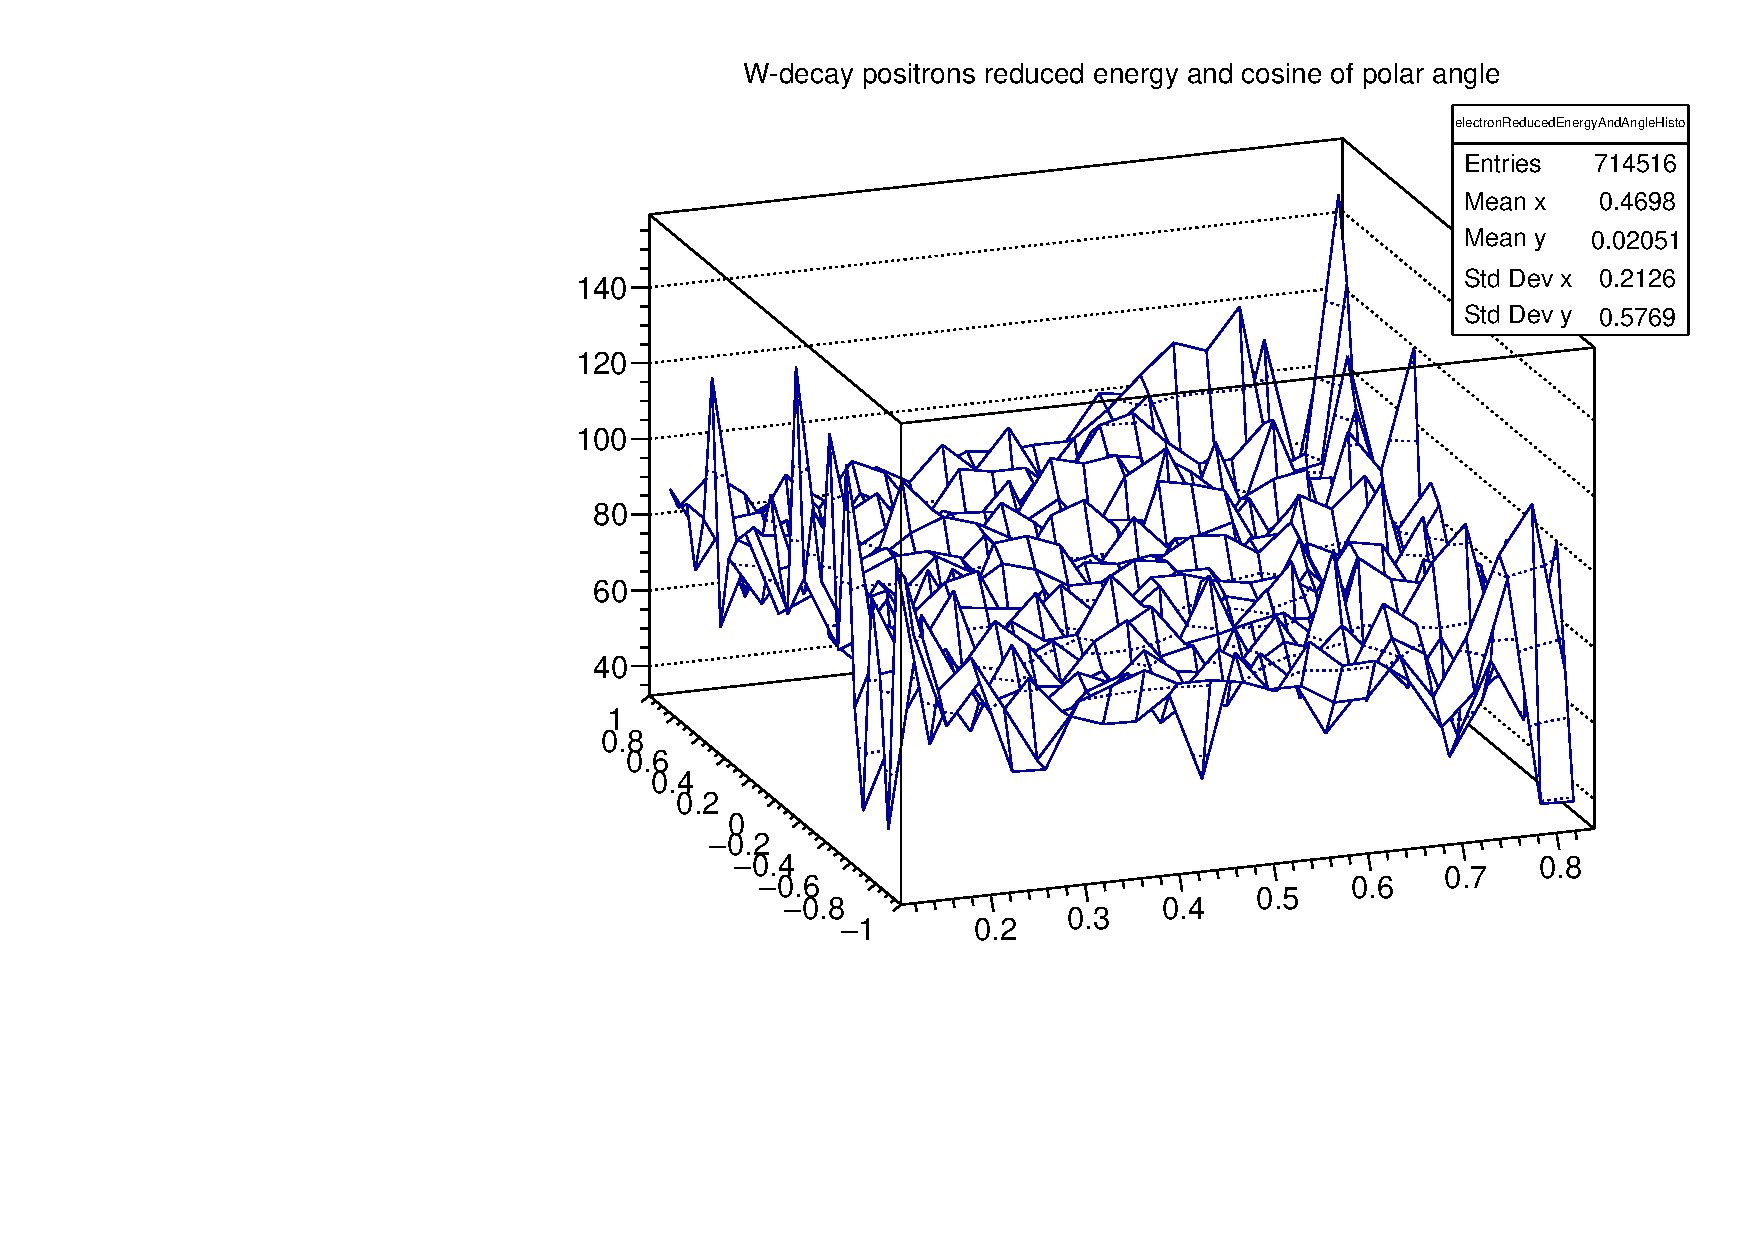
\includegraphics[width=0.7\textwidth]{02_Ratio_MC_An_zoom.pdf}
 \caption{Zoom of the ratio of the distribution simulated and analytic}
 \label{02_Energy_angle_ratio_zoom}
\end{figure}

In the end we can say that our work can start, because our data take in account the polarization effect.

\subsection{Other leptons simulations}

We have just started to stage, copy and Marlin also the files containing one muon or tau.

\section{Week 03}

\subsection{03/08/2015}

\textbf{Other leptons Whizard simulations}

We have copied and Marlin all the other simulations files with one leptons (muons or electrons) in the final state.\\
We would like to analyze the energy-angle distribution to understand if the boundary effect are due to some diagrams which interferes (only in the electrons case) or if they are due to something else.

\textbf{Likelihood fit}

After a lesson about the likelihood and how to fit an histogram by finding the minimum of the likelihood (thanks to Patrick), we started fitting our energy-angle distribution for the electrons with a model $S_0 + a f_1$, where $S_0$ is the standard model distribution and $f_1$ is a BSM correction.\\

We have started from two histograms of $S_0$ and $f_1$ with 200 bins in each dimension and reduced energy between 0.114246 and 1, and $cos\theta$ between -1 and 1 (obviously).\\ We have then normalized the distribution so we can use them as probability density function. So we have reproduced our distribution with these settings and use the likelihood formula:
\[L=-\sum_{events} log(S_0+a f_1) = -\sum_{bins} N_{bin} log(S_0+a f_1)\]
\[L'=-\sum N \frac{f_1}{S_0 + a f_1}  and  L''= \sum N \frac{f_1^2}{(S_0 + a f_1)^2}\]

where N is the number of entries in the selected bin of the montecarlo histogram, and $S_0$ and $f_1$ are the numbers of the entries in the histograms of the probability density function.

Then we could use the tangent method to find iteratively the minimum value (that we expect to be 0).
\[a_0 = a - \frac{L'(a)}{L''(a)}\]

and after all we can estimate the error with \[\sigma = \sqrt{\frac{1}{L''(a_0)}}\]

We have found some errors while calculating the Likelihood and its derivatives cause to the fact that $S_0$ and $f_1$ became very near to 0 in some points. We don't now how to solve yet.

\subsection{04/08/2015}

\textbf{TChain}

We have just discovered a new method to process a lot of Root files containing tree without using glob.
We simply need to define a TChain object:\\
mychain = TChain("MyTreeName")
where MyTreeName is the name of the trees inside the root files.\\
Then we can add all the root files to the chain by using:
mychain.Add("*.root")\\
and then we can loop on all the events dealing mychain as a tree.

\textbf{Likelihood fit part 2}

We found the problem in the code: strangely, if we look to the $S_0$ and $f_1$, we find that the bins (0,*) and (*,0) contains exactly 0 entries. So during the calculation of the derivatives we find several problems in dividing by zero. We solve the problem by simply don't consider these bins. The result is pretty strange because, starting with an initial value of a=0.1 we obtain a result of $a=0.2 \pm 0.01$ with a first derivative very close to zero. This result is only quite reasonable because we expect something close to zero, with 0 into the errorbar.

After a little time we found out that the first bins (*,0) and (0,*) and the last bins (*,201) and (201,*) are the overflow and the underflow of the histograms, so we need to use the method GetBinContent on the bin between 1 and 200 in both directions. The result hasn't changed and we tried to plot the marginal distributions. But this result is not satisfactory.

\section{Week 04}

\subsection{10/08/2015}

\textbf{Searching among the reconstructed particles}

We have just started to write some macros and to plot some histograms to understand how to find the electron coming from the primary vertex. The result are described in the next subsection.

\subsection{11/08/2015}

\textbf{Meeting with Patrick and Patrizia}

We have had a meeting in which we have talked about some things:

\begin{itemize}
\item Acceptance and efficiency: We need to produce some plots to understand what is the efficiency of our algorithm that finds the right electron. In addition we could understand which is the acceptance of the detector (in particular we expect that the acceptance is flat in the energy and have a plateau in cosTheta and two tails near 1 and -1.
\item Bremsstrahlung correction: We need to correct the bremsstrahlung of the electrons by adding the energy of the photons radiated by the electron. One way is to select the photons in a cone around the electron. A better way is to select the photons radiated parallel to the electron track: we could select the vertex and the end point of the electron and we could add all the photons with angle theta and phi compatible with the electron.
\item Sensitivity in measuring the energy and the Pt of the electron: we need to produce some plots to take in account the smearing produced by the uncertainty in measuring energy and transverse momentum.
\item Start writing code with classes and function
\end{itemize}

\textbf{New organization of the code}

The code is now written using classes and function.
We have defined a class "Particle" and a class "Jet" which contain the information we want in our object and some useful methods (like a correction which apply a bremsstrahlung correction to the electrons by adding the photons in a cone).

\textbf{Finding the correct electron}

We are searching for the best algorithm to find the correct a electron between the reconstructed particles. There are some ways to find this electron starting from the request that this electron is isolated. To see if the method is good or not we always plot the difference in energy and in angle between the montecarlo electron and the reconstructed electron.

\begin{itemize}
\item Pt rel: we loop on all the electrons, and, for each electron we select the jet respect to which the electron has the minimum Pt. The correct electron is, then, the electron with the highest "minimum Pt rel".\\
\item Pt rel to the closest jet: we loop on all the electrons and we search for the the closest jet, and the we calculate the Pt respect to that jet. The correct electron is, then, the electron with the highest Pt rel to the closest Jet.\\
\item Energy in a cone: we loop on all the electron and we find that one with the minimum energy inside a cone with fixed angle (typically 10 degrees).\\
\item Particle in a cone: we loop on all the electron and we find that one with the maximum distance from the closest particle (and we can add some cut, for instance we can require the closest charged particle or the closest particle different from a photon or an electron).
\end{itemize} 

In addition we use the kinematic constrain (Energy lower then 13 GeV) to select only the electrons with an energy lower than 10 GeV (to take in account the experimental uncertainty. This have two effects: improve the efficiency and reduce the computation time.

Results:???

\subsection{13/08/15}

We changed our approach, restarting our study considering the muons sample. This makes our work simpler, because muons have less background than electrons and usually loose less energy before their detection. Besides, there are far fewer muons than electrons in every event.

\textbf{Matching algorithm calibration}
We would like to find an algorithm to decide wether a reconstructed (RC) muon matches the W-decay Monte Carlo (W-MC) one. We decided to use, as discriminant variable, the angle between the relative momenta. To set the threshold value, we considered the events with three or more RC muons\footnote{Which are about 2\% of the events, whereas there are two RC muons in 20\% of the events and no RC muons in 1\% of cases.} (where is more probable that there is a muon that matches the W-MC one).
%\part*{Appendici}
%
%\appendix
%\cleardoublepage  
%\section{Relazione sul trigger di Schmitt}
%\includepdf[pages={1-10}]{relazione_trigger_di_schimitt.pdf} 
%
%\section{Relazione sull'effetto Ramsauer-Townsand}
%\includepdf[pages={1-5}]{relazione_ramsauer.pdf} 
%
%\section{Relazione sull'effetto fotoelettrico}
%\includepdf[pages={1-4}]{relazione_fotoelettrico.pdf} 


%final
\end{document}